\documentclass{beamer}
\usepackage{listings}
\lstset{
%language=C,
frame=single, 
breaklines=true,
columns=fullflexible
}
\usepackage{subcaption}
\usepackage{url}
\usepackage{tikz}
\usepackage{tkz-euclide} % loads  TikZ and tkz-base
%\usetkzobj{all}
\usetikzlibrary{calc,math}
\usepackage{float}
\newcommand\norm[1]{\left\lVert#1\right\rVert}
\providecommand{\pr}[1]{\ensuremath{\Pr\left(#1\right)}}
\providecommand{\sbrak}[1]{\ensuremath{{}\left[#1\right]}}
\providecommand{\brak}[1]{\ensuremath{\left(#1\right)}}
\providecommand{\fourier}{\overset{\mathcal{F}}{ \rightleftharpoons}}
\providecommand{\abs}[1]{\left\vert#1\right\vert}
\renewcommand{\vec}[1]{\mathbf{#1}}
\usepackage[export]{adjustbox}
\usepackage[utf8]{inputenc}
\usepackage{amsmath}
\usetheme{Boadilla}

\title{GATE EC 2017- Q.8}
\author{Tanmay Goyal - AI20BTECH11021}

\date{}

\begin{document}

\begin{frame}
\titlepage
\end{frame}
\begin{frame}
\frametitle{Question}
\begin{flushleft}
The input $x(t)$ and output $y(t)$ of a continous time signal are related as:
\begin{align}
    y(t) = \int_{t-T}^tx(u)\,du
\end{align}
The system is:
\begin{enumerate}
    \item Linear and Time-variant
    \item Linear and Time-invariant
    \item Non-Linear and Time-variant
    \item Non-Linear and Time-invariant
\end{enumerate}
\end{flushleft}
\end{frame}

\begin{frame}[fragile]
\frametitle{Linear Systems and Time Invariant Systems}

\begin{flushleft}
\begin{definition}
We say that a system is\textbf{ linear} if and only if it follows the Principle of Superposition, i.e Law of Additivity and Law of Homogeneity.
\label{L}
\end{definition}
          \end{flushleft}
    \begin{flushleft}
    \begin{definition}
A system is said to be \textbf{time invariant} if the output signal does not depend on the absolute time, i.e a time delay on the input signal directly equates to the delay in the output signal.
\label{T}
\end{definition}
\end{flushleft}
\end{frame}


\begin{frame}[fragile]
\frametitle{Lemma}
\begin{flushleft}
\begin{lemma}
The system relating the input signal $x(t$) and output signal $y(t)$, given by 
\begin{align}
     y(t) = \int_{t-T}^tx(u)\,du
\end{align}
is linear and time invariant in nature.
\end{lemma}
\end{flushleft}

\end{frame}

\begin{frame}{fragile}
\frametitle{Proof: Law of Additivity}

\begin{flushleft}
Let the input signals be $x_1(t)$ and $x_2(t)$, and their corresponding output signals be $y_1(t)$ and $y_2(t)$, then:
\begin{align}
    y_1(t) = \int_{t-T}^tx_1(u)\,du\\
    y_2(t) = \int_{t-T}^tx_2(u)\,du\\
    y_1(t) + y_2(t) = \int_{t-T}^t[x_1(u) + x_2(u)]\,du
    \label{1}
\end{align}
\end{flushleft}

\end{frame}
\begin{frame}{fragile}
\frametitle{Proof: Law of Additivity}

\begin{flushleft}
Now, consider the input signal of $x_1(t) + x_2(t)$, then the corresponding output signal is given by $y'(t)$:
\begin{align}
    y'(t) = \int_{t-T}^t[x_1(u) + x_2(u)]\,du
    \label{2}
\end{align}
Clearly, from \eqref{1} and \eqref{2}:
\begin{align}
    y'(t) = y_1(t) + y_2(t)
\end{align}
Thus, the Law of Additivity holds.\\

\end{flushleft}
    
\end{frame}

\begin{frame}
    \frametitle{Proof: Law of Homogeneity}
    \begin{flushleft}
      Consider an input signal $kx(t)$, where $k$ is any constant. Let the corresponding output be given by $y'(t)$, then:
\begin{align}
    y'(t) = \int_{t-T}^t kx(u)\,du\\
    = k\int_{t-T}^t x(u)\,du\\
     = ky(t)
     \label{3}
\end{align}
Clearly, from \eqref{3},
\begin{align}
    y'(t) = ky(t)
\end{align}
Thus, the Law of Homogeneity holds.\\
  \end{flushleft}
\end{frame}

\begin{frame}
    \frametitle{Proof}
    \begin{flushleft}
    Since both the Laws hold, the system satisfies the Principle of Superposition, and is thus, a \textbf{linear system}.\\
    \end{flushleft}
\end{frame}

\begin{frame}
    \frametitle{Proof: Time Invariance}
    \begin{flushleft}
    To check for time-invariance, we would introduce a delay of $t_0$ in the output and input signals.\\
Delay in output signal:
\begin{align}
    y(t-t_0) = \int_{t-t_0-T}^{t-t_0} x(u)\,du
    \label{4}
\end{align}
    \end{flushleft}
\end{frame}

\begin{frame}
    \frametitle{Proof: Time Invariance}
    \begin{flushleft}
    Now, we consider an input signal with a delay of $t_0$, given by $x(t-t_0)$, and let the corresponding output signal be given by $y'(t)$, then:
\begin{align}
    y'(t) = \int_{t-T}^{t} x(u-t_0)\,du
\end{align}
Substituting $a = u-t_0$:
\begin{align}
    y'(t) = \int_{t-t_0-T}^{t-t_0} x(a)\,da
    \label{5}
\end{align}
Clearly, from \eqref{4} and \eqref{5}:
\begin{align}
    y'(t) = y(t-t_0)
\end{align}
Thus, the system is \textbf{time-invariant}.\\

 Thus, \textbf{2) Linear and Time- invariant} is the correct answer.
    \end{flushleft}
\end{frame}

\begin{frame}
    \frametitle{Impulse response}
    \begin{flushleft}
    Since the given system is an LTI system, it would possess an impulse response $h(t)$, which is the output of the system when the input signal is the Impulse function, given by $\delta(t)$. Thus,
\begin{align}
    h(t) = \int_{t-T}^{t} \delta(u)du
\end{align}
    \end{flushleft}
\end{frame}
\begin{frame}
    \frametitle{Impulse function}
    \begin{flushleft}
    The Impulse function can be loosely defined as:
\begin{align}
    \delta(t) = 
    \begin{cases}
\infty & t = 0\\
0 & otherwise
\end{cases}
and \int_{-\infty}^\infty \delta(t)dt  = 1
\end{align}
    \end{flushleft}
\end{frame}
\begin{frame}
    \frametitle {Impulse response}
    \begin{flushleft}
    Since the Impulse function is zero everywhere aside from $t = 0$ , the non-zero value of integration is a result of $\delta(0)$. Thus, we can say $h(t)$ will be non-zero only if the limits of integration would include $t=0$, i.e:
\begin{align}
    h(t) = 
    \begin{cases}
    \int_{t-T}^{t} \delta(u)du & t-T<0 ; t>0\\
    0 & otherwise
    \end{cases}
    \end{align}
    \begin{align}
h(t) = 
    \begin{cases}
    1 & 0<t<T\\
    0 & otherwise
    \end{cases}
    \label{H}
\end{align}
    \end{flushleft}
\end{frame}

\begin{frame}
    \frametitle{Impulse response in terms of unit step signal}
    \begin{flushleft}
    The unit step signal, $u(t)$, is given by:
\begin{align}
    u(t) = 
    \begin{cases}
    1 & t\geq0\\
    0 & otherwise
    \end{cases}
    \label{u(t)}
\end{align}
On time-shifting $u(t)$ by T, we get:
\begin{align}
     u(t - T) = 
    \begin{cases}
    1 & t-T\geq 0\\
    0 & otherwise
    \end{cases}
    = 
    \begin{cases}
    1 & t\geq T\\
    0 & otherwise
    \end{cases}
    \label{u(t-T)}
\end{align}
On subtracting \eqref{u(t)} and \eqref{u(t-T)}, we get our impulse response $h(t)$ in terms of the unit step signal:
\begin{align}
    h(t) = u(t) - u(t-T)
\end{align}
    \end{flushleft}
\end{frame}

\begin{frame}
    \frametitle {Impulse response in terms of the unit rectangular function}
    \begin{flushleft}
    The unit rectangular signal, $rect(t)$ is given by:
\begin{align}
    rect(t) = 
    \begin{cases}
    1 & \frac{-1}{2} \leq t \leq \frac{1}{2} \\
    0 & otherwise
    \end{cases}
    \label{rect}
\end{align}
We can obtain the impulse response $h(t)$ in terms of $rect(t)$ using time scaling and shifting as follows:
\begin{align}
    rect\brak{\frac{t}{\tau}} = 
    \begin{cases}
    1 & \frac{-1}{2} \leq \frac{t}{\tau} \leq  \frac{1}{2}\\
    0 & otherwise
    \end{cases}
     = 
     \begin{cases}
     1 & \frac{-\tau}{2} \leq t \leq  \frac{\tau}{2}\\
    0 & otherwise
     \end{cases}
    \end{align}
    Subsituting $\tau = T$:
    \begin{align}
    rect\brak{\frac{t}{T}} = 
    \begin{cases}
    1 & \frac{-T}{2} \leq t \leq \frac{T}{2}\\
    0 & otherwise
    \end{cases}
    \end{align}
    \end{flushleft}
\end{frame}
\begin{frame}
    \frametitle{Impulse response in terms of the unit rectangular function}
    \begin{flushleft}
      Now, we want to right-shift the signal by $\frac{T}{2}$:
    \begin{align}
    rect\brak{\frac{1}{T}\brak{t - \frac{T}{2}}} = 
    \begin{cases}
    1 &  0 \leq t \leq T\\
    0 & otherwise
    \end{cases}
     = h(t)
\end{align}
Since the time shifting is to be performed on the variable $t$ and not $\frac{t}{T}$\\
    \end{flushleft}
\end{frame}
\begin{frame}
    \frametitle{Fourier Transform of rectangular function}
    \begin{flushleft}
    \begin{align}
    rect(t) \fourier Y(f)
    \end{align}
    \begin{align}
    Y(f) = \int_{-\infty}^\infty rect(t)e^{-j2\pi f t}\,dt
    \label{Fourier}
\end{align}
From \eqref{rect}, we can write \eqref{Fourier} as:
\begin{align}
   Y(f) = \int_{-\infty}^\frac{-1}{2} 0\,dt + \int_{\frac{-1}{2}}^\frac{1}{2} e^{-j2\pi ft}\,dt + \int_\frac{1}{2}^\infty 0\,dt
    = \frac{e^{j\pi f} - e^{-j \pi f}}{j2\pi f}\\
      = \frac{\sin (\pi f)}{\pi f}
       = sinc( f)
\end{align}
where $sinc(t)$ is defined as:
\begin{align}
    sinc(t) = 
    \begin{cases}
    1 & t = 0\\
    \frac{\sin(\pi t)}{\pi t} & otherwise
    \end{cases}
\end{align}
    \end{flushleft}
\end{frame}
\begin{frame}
    \frametitle{Properties of Fourier Transform}
    \begin{flushleft}
    Let the Fourier Transform of a signal $x(t)$ be $X(f)$.
\begin{align}
    x(t) \fourier X(f)
\end{align}
When the signal $x(t)$ is time shifted by $t_0$, the resultant Fourier Transform is given by:
\begin{align}
    x(t \pm t_0) \fourier X(f)e^{\pm j2\pi ft_0}
    \label{shift}
\end{align}
And when the signal $x(t)$ is time scaled by $\alpha$, the resulting Fourier Transform is given by:
\begin{align}
    x(\alpha t) \fourier \frac{1}{\abs{\alpha}}X\brak{\frac{f}{\alpha}}
    \label{scale}
\end{align}
    \end{flushleft}
\end{frame}
\begin{frame}
    \frametitle{Fourier Transform of impulse response}
    \begin{flushleft}
    \begin{align}
    rect(t) \fourier sinc( f)
\end{align}
Using \eqref{shift}:
\begin{align}
    rect\brak{t - \frac{T}{2}} \fourier sinc( f)e^{-j(2 \pi f)\frac{T}{2}}\\
    rect\brak{t - \frac{T}{2}} \fourier sinc( f)e^{-j \pi f T}
\end{align}
Using \eqref{scale},
\begin{align}
    rect\brak{\frac{1}{T}\brak{t - \frac{T}{2}}} \fourier \frac{1}{\frac{1}{\abs{T}}}sinc\brak{\frac{ f }{\frac{1}{T}}}e^{\frac{-j \pi f T}{T}}\\
    h(t) \fourier Tsinc\brak{ f T}e^{-j\pi f}\\
    \therefore H(f)  = Tsinc\brak{ f T}e^{-j\pi f}
\end{align}
    \end{flushleft}
\end{frame}

\begin{frame}
\frametitle{Cosine input signal}    
\begin{flushleft}
Consider an input signal of $x(t) = \cos{2\pi f_0t}$. The Fourier Transform of $x(t)$ is given by:
\begin{align}
    x(t) = \cos{2\pi f_0t} \fourier \frac{1}{2}\sbrak{\delta(f - f_0) + \delta(f + f_0)}
\end{align}
using the fact that 
\begin{align}
    \cos{2\pi f_0 t} = \frac{e^{j2\pi f_0 t} + e^{-j2\pi f_0 t}}{2}
\end{align} and the Fourier Transform of $e^{\pm j2\pi f_0 t}$ is given by:
\begin{align}
    e^{\pm j2\pi  f_0 t} \fourier \delta(f \mp f_0)
    \label{FT}
\end{align}
\end{flushleft}
\end{frame}

\begin{frame}
    \frametitle{Output Signal}
    \begin{flushleft}
The output signal will be given by:
\begin{align}
    y(t) = \int_{t-T}^t \cos{2\pi f_0u}\,du\\
     = \frac{1}{2\pi f_0}\sbrak{\sin{2\pi f_0t}- \sin2\pi f_0({t-T})}\\
      = \frac{\sin\pi f_0 T}{\pi f_0} \sbrak{\cos2\pi f_0 \brak{t - \frac{T}{2}}}\\
      = Tsinc( f_0 T)\cos2\pi f_0\brak{t - \frac{T}{2}}
      \label{output}
\end{align}
    \end{flushleft}
\end{frame}
\begin{frame}
    \frametitle{Fourier Transform of output signal}
    \begin{flushleft}
    The Fourier transform of $\cos2\pi f_0\brak{t - \frac{T}{2}}$ can be obtained using \eqref{scale} and \eqref{shift} as follows:

\begin{align}
    \cos t = \frac{1}{2}\sbrak{e^{jt} + e^{-jt}}\\
    \cos t \fourier \frac{1}{2}\sbrak{\delta\brak{f - \frac{1}{2\pi}} + \delta\brak{f + \frac{1}{2\pi}}}\\
    \cos\brak{t - \frac{T}{2}} \fourier \frac{1}{2}\sbrak{\delta\brak{f - \frac{1}{2\pi}} + \delta\brak{f + \frac{1}{2\pi}}} e^{j\pi fT}\\
    \cos2\pi f_0\brak{t - \frac{T}{2}} \fourier \frac{1}{2\pi f_0}\frac{\delta(\frac{f}{2\pi f_0} - \frac{1}{2\pi}) + \delta(\frac{f}{2\pi f_0} + \frac{1}{2\pi})}{2} e^{j\pi \frac{f}{2\pi f_0}T}\\
    \cos2\pi f_0\brak{t - \frac{T}{2}} \fourier\frac{1}{4\pi f_0}\brak{\delta\brak{\frac{f - f_0}{2\pi f_0}} + \delta\brak{\frac{f + f_0}{2\pi f_0}}}e^{j\pi \frac{f}{2f_0}T}
\end{align}

    \end{flushleft}
\end{frame}

\begin{frame}
\frametitle{Fourier Transform of output signal}
The Fourier Transform of the output signal $y(t)$ from \eqref{output} is given by:
 \begin{align}
     y(t) \fourier \frac{Tsinc( f_0 T)}{4\pi f_0}e^{j\pi \frac{f}{2f_0}T}\brak{\delta\brak{\frac{f - f_0}{2\pi f_0}} + \delta\brak{\frac{f + f_0}{2\pi f_0}}}\\
     y(t) \fourier ke^{j\pi \frac{f}{2f_0}T}\brak{\delta\brak{\frac{f - f_0}{2\pi f_0}} + \delta\brak{\frac{f + f_0}{2\pi f_0}}}
 \end{align}
 where $k = \frac{Tsinc( f_0T)}{4\pi f_0}$.
\end{frame}
\begin{frame}
    \frametitle{Fourier Transform of output signal}
    \begin{flushleft}
    Substituting $2\pi f_0 = 1$ and $T = 1$:
 \begin{align}
     y(t) \fourier ke^{j\pi^2f}\brak{\delta\brak{f - \frac{1}{2\pi}} + \delta\brak{f + \frac{1}{2\pi}}}\\
     y(t) \fourier ke^{j\frac{\pi}{2}}\delta\brak{f - \frac{1}{2\pi}} +ke^{j\frac{-\pi}{2}}\delta\brak{f + \frac{1}{2\pi}}
 \end{align}
 using the multiplication property of the Delta function:
 \begin{align}
     x(t)\delta(t - t_1) = x(t_1)\delta(t - t_1)
 \end{align}
 Since , $e^{j\frac{\pi}{2}} = j$ and $e^{-j\frac{\pi}{2}} = -j$, we finally get:
 \begin{align}
 y(t) \fourier kj\sbrak{\delta\brak{f - \frac{1}{2\pi}} - \delta\brak{f + \frac{1}{2\pi}}}
 \end{align}
    \end{flushleft}
\end{frame}
\begin{frame}
\frametitle{Output signal}
\begin{flushleft}
\begin{align}
    y(t) \fourier kj\sbrak{\delta\brak{f - \frac{1}{2\pi}} - \delta\brak{f + \frac{1}{2\pi}}}
\end{align}
Clearly, the Fourier transform of $y(t)$ can  be  manipulated  to  represent  a  sinusoidal  wave,  which  is given by:
 \begin{align}
     sin(t) \fourier \frac{-j}{2}\sbrak{\delta\brak{f-\frac{1}{2\pi}} - \delta\brak{f + \frac{1}{2\pi}}}
 \end{align}
\end{flushleft}
\end{frame}
\begin{frame}
    \frametitle {Fourier Transform of Impulse response: Graph}
    The attenuation happens for the same value of $f$, as depicted in the graphs of the Fourier Transforms below.
    \begin{columns}
\begin{column}{0.5\textwidth}
\begin{figure}
\begin{flushleft}
\centering
 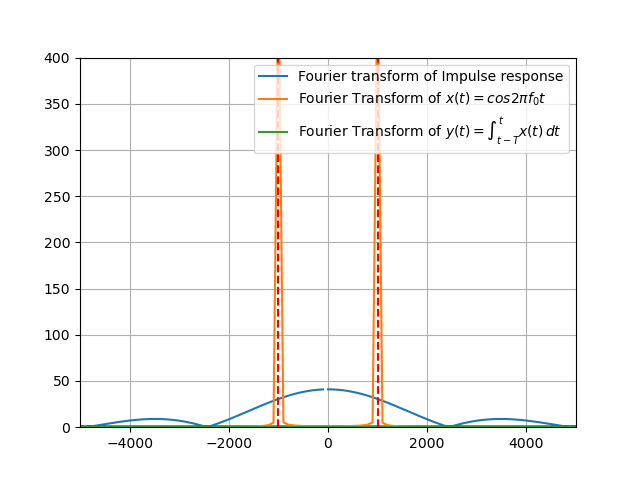
\includegraphics[width=\columnwidth]{graphs/fourier_impulse_response.png}
 \caption{Fourier Transform of impulse response and example input and output signal}
    \end{flushleft}
    \end{figure}
    \end{column}
   \begin{column}{0.5\textwidth}
    \begin{figure}
\begin{flushleft}
\centering
 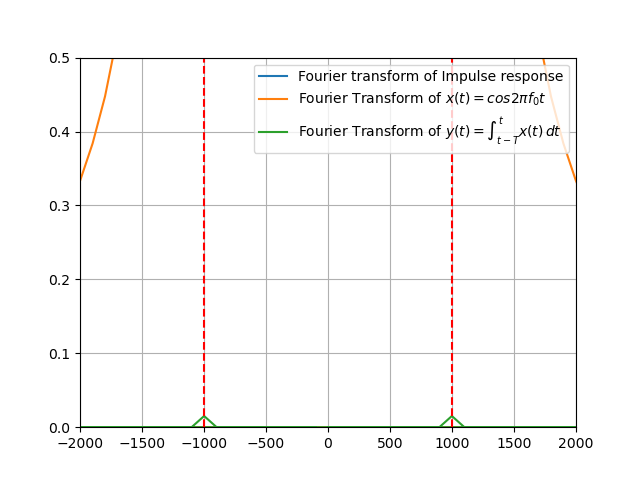
\includegraphics[width=\columnwidth]{graphs/fourier_impulse_response_zoomed.png}
 \caption{Fourier Transform of impulse response and example input and output signal zoomed in}
 \end{flushleft}
 \end{figure}
    \end{column}
    \end{columns}
\end{frame}

\begin{frame}
  \frametitle{Graphs: Input and Output signals}
 \begin{columns}
\begin{column}{0.5\textwidth}
\begin{figure}
\begin{flushleft}
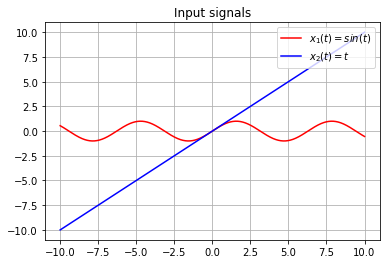
\includegraphics[width=\columnwidth]{graphs/input_signals.png}
 \caption{$x_1(t) = \sin{t}$ and $x_2(t) = t$}
\end{flushleft}
\end{figure}
\end{column}
\begin{column}{0.5\textwidth}
\begin{figure}
\begin{flushleft}
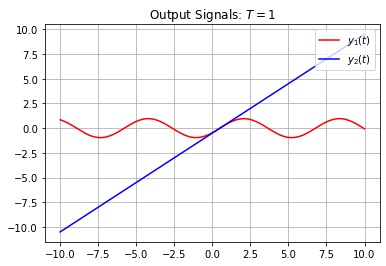
\includegraphics[width=\columnwidth]{graphs/output_signals.png}
 \caption{$y_1(t)$ and  $y_2(t)$}
\end{flushleft}
\end{figure}
\end{column}
\end{columns}
\end{frame}

\begin{frame}
  \frametitle{Graphs: Laws of Additivity and Homogeneity}
 \begin{columns}
\begin{column}{0.5\textwidth}
\begin{figure}
\begin{flushleft}
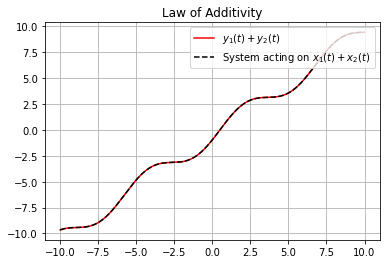
\includegraphics[width=\columnwidth]{graphs/law_of_additivity.png}
 \caption{Law of Additivity}
\end{flushleft}
\end{figure}
\end{column}
\begin{column}{0.5\textwidth}
\begin{figure}
\begin{flushleft}
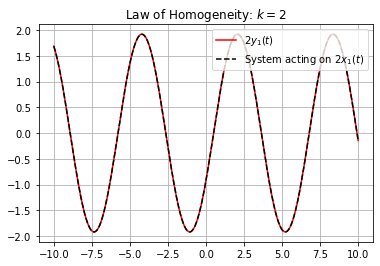
\includegraphics[width=\columnwidth]{graphs/law_of_homogeneity.png}
 \caption{Law of Homogeneity}
\end{flushleft}
\end{figure}
\end{column}
\end{columns}
\end{frame}

\begin{frame}
    \frametitle{Graphs: Time Invariance}
    \begin{figure}
\begin{flushleft}
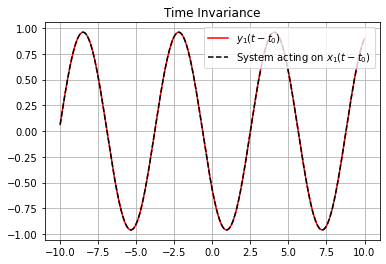
\includegraphics[width=\columnwidth]{graphs/time_invariance.png}

 \caption{Time invariance}
\end{flushleft}
\end{figure}
\end{frame}
\end{document}
